Our second contribution is to minimize the above heterogeneity using the
Charm++ load balancing strategies.  We first observed the working of existing load
balancers like \emph{RefineLB} \& \emph{GreedyLB} to evaluate the its effect in
minimizing the heterogeneity. 
 
\subsection{Existing Load-balancers} 
Load balancing is a technique of distributing computational and communication
load evenly across processors of a parallel machine so that no single processor
is overloaded.  Charm++ implements a generic, measurement-based load balancing
framework which automatically instruments all Charm++ objects, collects
computation load and communication structure during execution and stores them
into a load balancing database.  Charm++ then provides a collection of load
balancing strategies whose job it is to decide on a new mapping of objects to
processors based on the information from the database.  These strategies work
under the assumption that objects in a Charm++ application tend to exhibit
temporal correlation in their computation and communication patterns, i.e.
future can be predicted to some extent using the collected data, allowing
effective measurement-based load balancing without application-specific
knowledge. Following are the two widely used load balancing strategies:

\subsubsection{RefineLB}
The objective of this strategy is to move objects away from the most overloaded
processors to less overloaded ones so as to reach an average load on each
processors. Algorithm~\ref{alg:refine} shows the pseudo-code for this strategy:

\begin{algorithm}
 \KwData{V$_t$:(the set of objects; V$_p$ (the set of processors)}
 \KwResult{Map:V$_t \rightarrow $ V$_p$ (An object mapping) }
 // build heap \;
  ProcessorHeap heavyProcs(V$_p$)\;
  Set *lightProcs\;
  \While{!done} {
    donor =   heavyProcessors$\rightarrow$deleteMax()\;
    \While{ligthProcs} {
      (obj, lightProc)  $\leftarrow$ BestObjFromDonor(donor)\;
      \If{obj.load + lightProc.load $>$ avg\_load} {
        continue\;
      } 
      \If{obj\_obtained} {
        break\;
      }
      deAssign(obj, donor)\;
      assign(obj, lightProc)\;
    }
  }
 \caption{RefineLB Pseudocode}
 \label{alg:refine}
\end{algorithm}

 As evident from the above algorithm that it tries to migrate objects based on
 a global average which is computed as the average of each processor's load.
 As a result it restricts the number of migration which is otherwise possible.
 At lower power cap  the opportunity for objects migration will be more due to
 increased heterogeneity.  But this strategy being dependent on a global metric
 which may not change much at lower power caps.

\subsubsection{GreedyLB}
This uses a greedy algorithm that always assigns the heaviest object (load-wise) to the
least loaded processor. 

\begin{algorithm}
 \KwData{V$_t$:(the set of chare objects; \\ V$_p$ (the set of processors; \\ G$_p$ (the background load of processors) // due to non-migratable objects, etc.)}
 \KwResult{Map:V$_t \rightarrow $ V$_p$ (An object mapping) }

 // build heap of size equal to the number of objects \;
 ObjectHeap objHeap($|$V$_t|$)\;
 // insert each element of Vt in objHeap\;
 V$_t\rightarrow$objHeap \; 
 MinHeap cpuHeap(P)\;
 //Initially processors are empty with only background load\; 

 cpuHeap$\leftarrow$G$_p$\;  
 \For{ i$\leftarrow$1 to nmigobj} {
    o$\leftarrow$ objHeap.deleteMax()\;
    donor$\leftarrow$cpuHeap.deleteMin()\;
    Assign c to donor and record it in Map\;
    donor.load += c.load // add object load of c to the donor\;
    cpuHeap.insert(donor) \;
    }
 \caption{GreedyLB Pseudocode}
 \label{alg:greedy}
\end{algorithm}

The assumption for object migration is that the time taken by the object to
execute on a processor will remain the same both before and after the
migration.  This assumption is valid at higher power caps because (1) all the
objects are of same size and (2) at higher power capping values the processors
are running at nearly the same frequencies and hence the time taken by a chare
to run any of them is nearly equal.  But this assumptions fall apart at lower
power caps because of the heterogeneity introduced between the processors and
as a result it may happen that the object time will differ after the migration.
Algorithm~\ref{alg:greedy} shows the corresponding pseudo-code.

\subsection{Design: Power Aware Load Balancer}
We have established the fact that current load-balancers in charm++ are not
power aware. Current Load Balancers do not load balance based on the individual
performance of the processor at lower power caps. We have also established that
there is a definite scope for improvement in execution time of the application
by minimizing the maximum idle and the average idle times of the processor.
Our motive behind the design was to make all the processors finish the
execution at the same point of time. This approach takes relative speeds of the
processors into consideration for balancing the load. We use the object time of
the chares
, which is defined as the time taken by the chare to run on a
particular processor, to measure the relative speeds of the processors. We
explain in the next section, the reason to choose object time for the load
balancing.  In this approach we try to average out the execution time by
assigning the load in such a way that each of them is assigned exactly that
much amount of load which helps all the PEs finish at almost the same time. 
%As it can be seen in the Figure \ref{fig:ideal} different PEs finish execution
%at different points of time. As per the motive of the design we make all the
%processors to finish at the same time. 
The following two equations explains our load distribution strategy.  

%\begin{figure}
%\centering
%\scalebox{.40} {
%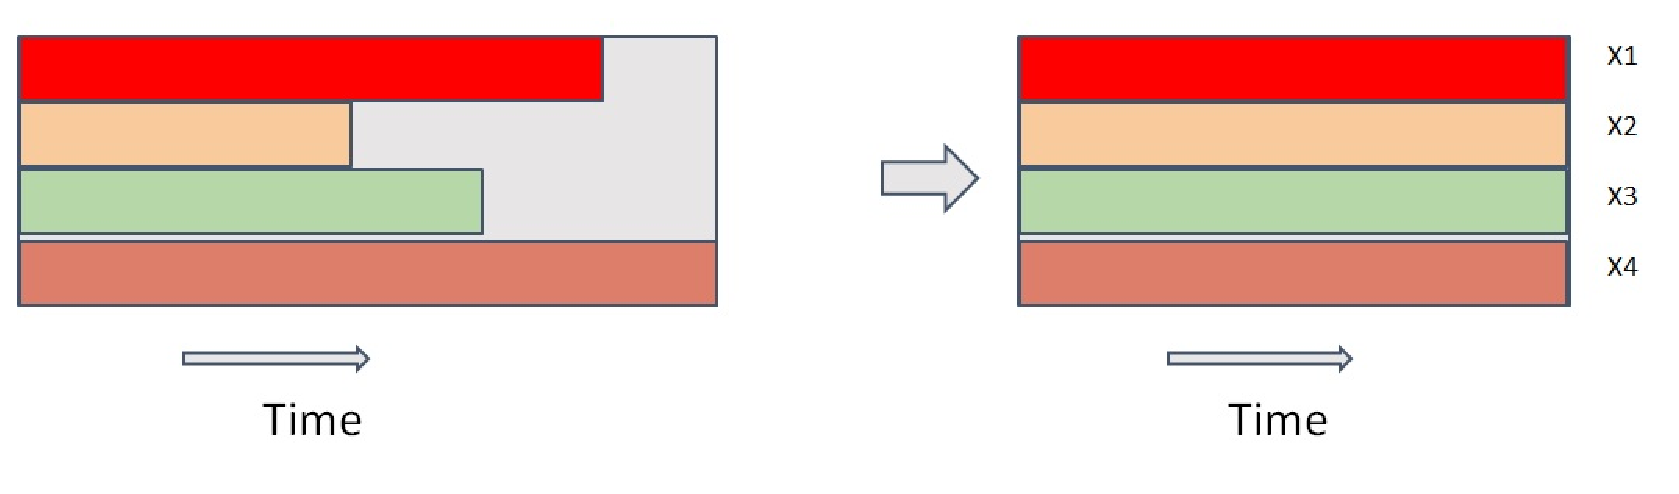
\includegraphics[scale=0.8]{Jacobi/EPS/time_diff.eps}
%}
%\caption{Expected Result of Power Aware Load Balancer}
%\label{fig:ideal}
%\end{figure}

    \begin{equation} \label{eq:3}
      (w_1x_1) = (w_2x_2) = (w_3x_3) = \dots = (w_nx_n) 
    \end{equation}
    \begin{equation} \label{eq:4}
      x_1 + x_2 + x_3 + \dots + x_n = N
    \end{equation}

  where, $w_i, 1 \leq i \leq n$ is the weight (in terms of times) for executing
  $x_i$ number of objects on processors PE$_i$ and $N$ is the total number of objects. 
  Before the load balancing all the x$_i$'s are the same as the Charm++
  runtime does an equal distribution of work on each processor. 
  The challenge is to choose the parameter $w_i$ in such a way that it correctly reflects the heterogeneity
  in performance of $i^{th}$ processor at lower power values and on the other hand  
  remain almost the same for higher power figures. We have chosen the metric of object time 
  for this purpose. The next subsection explains our  choice.
  %All the objects
  %have the same load/weight in terms of computation.  Each PE executes the same
  %number of objects before load balancing. Each PE before load balancing has
  %the same total load since each object has the same weight. 
  By using the above
  equation we get the proportionality based on which the number of objects need
  to be assigned while load balancing. For instance, processor PE$_1$ could
  be 2 times faster than PE$_2$ and P$_3$ could be 0.5 times faster than
  PE$_2$. In which case we will have the following proportionality: PE$_1$ :
  PE$_1$ : PE$_3$ = 2 : 1 : 0.5. Now based on this proportionality each processor is
  assigned such a load that everyone can finish their execution at the same
  point of time.  
  
  We use the both the equations (~\ref{eq:3}) and (~\ref{eq:4}) to determine
  $x_i$'s, $1 \leq i \leq n$, which is the new load for its respective
  processors that help finish all of them at almost the same time. The newly
  assigned load $x_i$ for each of the PEs is proportional to $w_i$ which we
  strive to reflect the relative speeds of the processors at a given power cap. 

\subsection{Selection of metric ``w''} 
We have considered processor idletime, processor background time
\footnote{Processor background time amounts to the overhead due to non
  migratable objects on that processor.} and processor object time \footnote{A
    processor's object time is defined as the sum of object times of all the
      objects executing on that processor.} as candidates for our selection.

      We measure these values for each processor at a power cap of 24W.
      Figures \ref{fig:idletime_bgtimevsproc} and \ref{fig:objtimevsproc} show
      the experimental plots.  The metric which has the maximum variance
      depicts the heterogeneity in the best possible way.  Percentage change
      between the maximum and minimum idle time was $0.35$, and the same for
      background time was $1.41$ and that of processor object time was $4.09$
      (This was partially due to a misbehavior of node0:core0 as seen in the
       Figure \ref{fig:objtimevsproc}).  Using the above observation we chose
      processor's object time as a metric for ``w'' because this shows the
      maximum variance at lower power caps. 
   

\begin{figure}
\begin{tabular}{cc}
  \scalebox{0.5}{
    \begin{tikzpicture}
  \begin{axis}[
   title = , 
   xlabel=  Core Ids,
   ylabel= Time (secs),
   ymax=2, ymin=0, xmax=60, xmin=0,
   x tick label style={black},
   grid=both
   ]
  \addplot table [x=PE, y=BG]{data2.dat};
  \addlegendentry {Overhead}
  \end{axis}
  \end{tikzpicture}
  }
& 
  \scalebox{0.5}{
    \begin{tikzpicture}
  \begin{axis}[
   title = , 
   xlabel=  Core Ids,
   ylabel= Time (secs),
   ymax=42, ymin=30, xmax=60, xmin=0,
   x tick label style={black},
   grid=both
   ]
  \addplot table [x=PE, y=I]{data2.dat};
  \addlegendentry {Idle Time}
  \end{axis}
  \end{tikzpicture}
  }
\\
\qquad (a) & \quad (b) \\
\end{tabular}
\caption{Idle and Overhead time over the cores at 24W power cap}
\label{fig:idletime_bgtimevsproc}
\end{figure}



\begin{figure}
\centering
  \scalebox{0.75}{
    \begin{tikzpicture}
    \begin{axis}[
     title = , 
     xlabel=  Core Ids,
     ylabel= Time (secs),
     ymax=58, ymin=11, xmax=60, xmin=0,
     x tick label style={black},
     grid=both
     ]
    \addplot table [x=PE, y=OBJ]{data2.dat};
    \addlegendentry {Collective Chare Time}
    \end{axis}
    \end{tikzpicture}
  }
\caption{{Processor object time on each processor at 24W power cap.}}
\label{fig:objtimevsproc}
\end{figure}
